\chapter{Análisis Experimental}
En esta sección se presenta la descripción de los escenarios, la plataforma de ejecución y el análisis experimental.

Este se divide en dos etapas, primero se realiza la configuración paramétrica para encontrar el mejor rendimiento del algoritmo y luego se realizan las pruebas donde se muestran los resultados y comparaciones.


\section{Desarrollo y Plataforma de ejecución }
Los algoritmos fueron desarrollados usando la biblioteca Malva que fue extendida en el código base para soportar la creación de nuevos hilos de ejecución para lograr el funcionamiento en paralelo.

Los escenarios fueron ejecutados en el cluster Fing.

Cluster: Es un conjunto de computadoras independientes conectadas para que trabajen integradas como un solo sistema. De esta forma se consigue un alto rendimiento en la ejecución de tareas. 

Cluster Fing: Es una infraestructura de alto desempeño, que brinda soporte en la resolución de problemas complejos que demandan un gran poder de computo.

Descripcion del hardware: 
\begin{itemize}
	\item 9 servidores de cómputo
	\subitem Quad core Xeon E5430, 2x6 MB caché, 2.66GHz, 1.333 MHz FSB.
	\subitem 8 GB de memoria por nodo.
	\subitem Adaptador de red dual (2 puertos Gigabit Ethernet).
	\subitem  Arquitectura de 64 bits.
	\subitem Servidor de archivos: 2 discos de 1 TB, capacidad ampliable a 10 TB.
	\subitem Nodos de cómputo: discos de 80 GB.
	\item Switch de comunicaciones
	\subitem Dell Power Connect, 24 puertos Gigabit Ethernet.
	\item Switch KVM (16 puertos) y consola.
	\item UPS APC Smart RT 8000VA.
\end{itemize}

\section{Ajuste paramétrico}
Se busca la mejor configuración inicial de los parámetros realizando pruebas experimentales con diferentes combinaciones.  
Los elementos que se ajustaran serán los siguientes:

\begin{itemize}
	\item Tiempo de simulación	
	\item Criterio de parada
	\item Tamaño de la población
	\item Probabilidad de mutación
	\item Probabilidad de cruzamiento
\end{itemize}

Para la realización de las pruebas se generan tres escenarios de tráfico diferentes para realizar las pruebas de configuración. En este caso no se utilizan datos recabados de la realidad como el tráfico especifico de las calles y el recorrido de las lineas de ómnibus. Esto para no sesgar el algoritmo a un caso en particular.
Los tres escenarios de tráfico son los siguientes:

\begin{itemize}
	\item Tráfico Bajo: 30 ómnibus y 500 vehículos	
	\item Tráfico Medio: 60 ómnibus y 1000 vehículos
	\item Tráfico Alto: 120 ómnibus y 2000 vehículos
\end{itemize}


En el ajuste paramétrico primero se define el tiempo de simulación y el criterio de parada, luego de establecidos se realizan las pruebas para todas las combinaciones de tasa de cruzamiento y mutación buscando los mejores valores para optimizar el algoritmo.

Al estar utilizando un cluster tenemos disponible tanto la métrica del tiempo real que llevo la ejecución, así como también el tiempo secuencial, es decir la suma del tiempo de procesamiento de todos los procesadores involucrados en la evaluación del algoritmo. 
Cuando se realicen comparaciones en los tiempos de ejecución se utilizara el tiempo secuencial que es independiente de la cantidad de procesadores utilizados en las pruebas. Las diferentes ejecuciones fueron realizadas sobre el Cluster utilizando entre 4 y 32 procesadores ya que por la naturaleza de recursos compartidos no siempre se tiene una cantidad igual  de procesadores libres y para estas pruebas el numero de procesadores no es relevante. Si lo sera cuando realicemos el análisis de eficiencia computacional que sera estudiando mas adelante.



\subsection{Pesos de la función fitness}

Para las siguientes pruebas la función fitness del algoritmo (\ref{eq:funcion_fitness}) tendrá los pesos x = y = 1. Esto da pesos equitativos tanto a ómnibus como a otros vehículos por lo que no existe prioridad para uno u otro. Mas adelante se realizaran experimentos con otras variantes.


\subsection{Tiempo de simulación}
Esto se refiere al tiempo que representa una simulación usando SUMO,  es un parámetro que se puede configurar y permite tener un mejor control sobre los tiempos totales de ejecución del algoritmo.

Se establece un tiempo de simulación de 4000 \emph{steps} (medida interna de tiempo del simulador SUMO). Este numero representa 66 minutos en la simulación, mientras el tiempo real de ejecución depende de la plataforma y de la cantidad de vehículos pero se encuentra entre los 5 a 20 segundos. Se tuvo en cuenta y validó que en cada escenario mas del 80 \% de los vehículos hayan completado la simulación, es decir llegado a sus destinos. Se realizaron 10 ejecuciones del algoritmo para cada uno de los tres tipos de tráfico comprobando que se cumplía el criterio.


\subsection{Criterio de parada}
Se elige como criterio de parada el número de generación, esto permite estandarizar las pruebas para una mejor comparación.

Para determinarlo se busca un compromiso entre un buen resultado y un tiempo de ejecución apropiado que no sea excesivo.

Para esto se decide que por un lado la ejecución del algoritmo deberá estar comprendida entre 1 y 24 horas, y además comprobar experimentalmente que el valor de fitness no tiene una gran variación en las ultimas 100 generaciones.

Se ejecutaron 10 ejecuciones del algoritmo por cada tipo de tráfico.

Luego de la realización de las pruebas se elige el número de 500 generaciones como criterio de parada.
En la siguiente gráfica se aprecia como el valor de fitness no presenta grandes variaciones luego de la generación 400 ademas el tiempo de ejecución real esta dentro del margen pautado. La gráfica no muestra todos los valores, solo algunos representativos para una mejor visualización.



\begin{figure}[h]
\centering
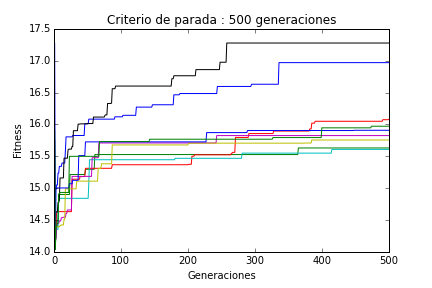
\includegraphics[width=0.7\linewidth]{Figures/criterio_parada}
\caption{Resumen representativo de ejecuciones del algoritmo para establecer el criterio de parada.}
\label{fig:criterio_parada}
\end{figure}



\subsection{Tamaño de la población}

Para la elección de la población se tendrán en cuenta 3 elementos. El valor de fitness encontrado, el tiempo de ejecución total y la plataforma de ejecución.

Dado que estamos ejecutando en el cluster y la máxima cantidad de procesadores que se pueden utilizar son 64 en un mismo nodo y teniendo en cuenta que la mejor distribución del trabajo es un elemento de población por procesador, se tiene que la máxima cantidad de población que estudiaremos sera 64.

Luego se eligen los valores 32 y 48 para completar el análisis teniendo en cuenta que no son lo suficientemente bajos y son valores con los que se obtiene una distribución más adecuada.

Se realizan 10 ejecuciones del algoritmo por cada tipo de tráfico y luego se obtiene el promedio de esos valores.

La siguiente tabla muestra los resultados obtenidos, como se aprecia no existen grandes diferencias en la elección de un número poblacional sobre otro. Por tanto se elige como número de población 32 teniendo en cuenta el tiempo de ejecución secuencial del algoritmo que como se aprecia es el menor. Se elige esta métrica por que aunque al ejecutar en paralelo el tiempo real que se puede obtener utilizando la máxima cantidad de procesadores para cada población son similares también se tiene en cuenta la disponibilidad y utilización de recursos que insume en el cluster fing. Por ejemplo obtener 64 procesadores para utilizar por un proceso en el cluster es algo que puede demorar varios días por la cantidad de otros procesos que también están funcionando en la plataforma y como se ve la ganancia que tenemos es mínima.

\begin{table}[h]
	\renewcommand{\arraystretch}{1.2}
	\caption{Comparación de fitness para distintas poblaciones}
	\label{table:parametro_poblacion}
	\centering
	\begin{tabular}{ccrrcp{2cm}}
		\hline
	    \multirow{2}{*}{\textbf{Población}}& & 
		\multicolumn{2}{c}{\textbf{Fitness}} \\
		\cline{3-4}
		& & {mejor} 
		& {promedio} 
		& \textbf{Tiempo ejecución serial (m)} \\
		\hline
		32 & & {17.28} & 16.37$\pm$0.5 & 10184$\pm$526\\
		48 & & {16.19} & 15.84$\pm$0.3 & 6772$\pm$256\\
		64 & & {17.27} & 16.46$\pm$0.6 & 4853$\pm$155\\
		\hline
	\end{tabular}
\end{table}





\subsection{Probabilidad de mutación y cruzamiento}

Los valores elegidos fueron:

\begin{itemize}
	\item Probabilidad de cruzamiento (pc):  0.5, 0.8, 1
	\item Probabilidad de  mutación (pm):  0.01, 0.05, 0.1
\end{itemize}

Se prueban las nueve combinaciones posibles de cruzamiento y mutación, para cada una se realizan 3 ejecuciones para el escenario con tráfico bajo, 3 con tráfico medio y 3 con tráfico alto.


 
 \begin{table}[h]
 	\renewcommand{\arraystretch}{1.2}
 	\caption{Combinaciones de probabilidad de cruzamiento(pc) y de mutación (pm)}
 	\label{table:parametro_mutacion_cruzamiento}
 	\centering
 	\begin{tabular}{p{1cm}p{1cm}p{3.5cm} }
 		\hline
 		$p_C$& 
 		$p_M$ & 
 		Fitness promedio  $\pm$ desviación estándar\\ 
 		\hline
 		0.5 & 0.01  &  16.09$\pm$0.30\\
 		0.5 & 0.05 &  15.60$\pm$0.17\\
 		0.5 & 0.1  &  16.16$\pm$0.42\\
 		0.8 & 0.01  &  16.04$\pm$0.55\\
 		0.8 & 0.05  &  15.85$\pm$0.32\\
 		0.8 & 0.1  &  16.08$\pm$0.34\\
 		1 & 0.01 &  16.08$\pm$0.45\\
 		1 & 0.05 &  15.82$\pm$0.34\\
 		1 & 0.1 &  16.04$\pm$0.25\\
 		\hline
 	\end{tabular}
 \end{table}
 
 
 

\begin{figure}[h]
	\centering
	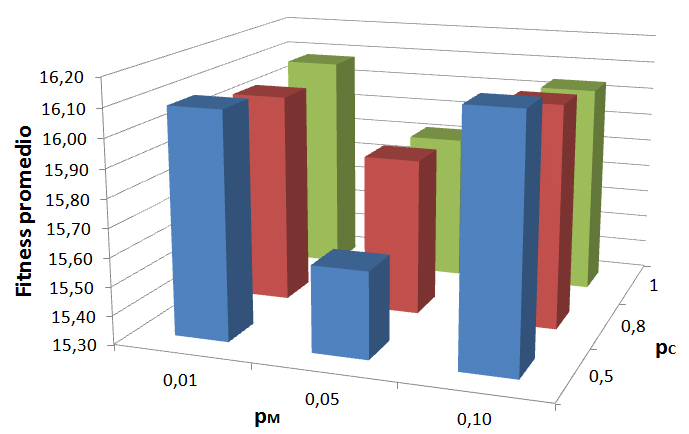
\includegraphics[width=0.7\linewidth]{Figures/grafica_mutacion_cruzamiento}
	\caption{Gráfica con combinaciones de probabilidad de cruzamiento(pc) y de mutación (pm)}
	\label{fig:grafica_mutacion_cruzamiento}
\end{figure}

Analizando la tabla y la gráfica se puede apreciar claramente que para una probabilidad de mutación de 0.05 se obtienen los peores resultados. Otro dato interesante es que no existe gran diferencia en el resto de las combinaciones.

Se comprueba que todas las muestras siguen la distribución normal  para poder aplicar el test de Student.

Siendo las hipótesis de la prueba ( u1 el promedio del  grupo 1 y u2 el del grupo 2) \newline
H0: u1  = u2  \newline
H1: u1 != u2 \newline

Si hacemos una comparación entre la combinación del mejor promedio (0.5-0.1) y del peor (0.5-0.05) con el test de Student obtenemos t(x) = 0.07 que nos indica que para un nivel de significancia de  0,1 la hipótesis nula es rechazada por lo tanto existe evidencia estadística para elegir la combinación con el mejor promedio (0.5-0.1) sobre la combinación con el peor promedio (0.5-0.05) para la ejecución del algoritmo.

Para comprobar si es la mejor opción  se toman las dos combinaciones con el mejor promedio (0.5-0.1) y (0.5-0.01) obteniendo en el test Student t(x) = 0.71 que nos indica que no existe una diferencia significativa entre ambas muestras por lo que elegir una sobre otra no implicaría grandes beneficios.

En tal sentido podríamos elegir cualquiera de las dos, en este caso se elige  la combinación (0.5-0.01) por su buen promedio y baja desviación estándar.



\section{Descripción de escenarios}
En esta sección se presentan los escenarios que serán evaluados, el primero es el escenario base que representa la realidad actual y el segundo un escenario alternativo que contiene modificaciones con el objetivo de mejorar la realidad.

\subsection{Caso base o Realidad actual del corredor}
Esto representa la situación actual en términos de tráfico, red vial y sincronización de semáforos del corredor Garzón. El objetivo es obtener datos precisos para realizar una simulación de la realidad y poder obtener datos para comparar con los resultados del algoritmo. 

Se valida su correctitud comparando los tiempos obtenidos en la simulación con tiempos obtenidos in-situ de los recorridos de ida y vuelta para los vehículos. Para el caso de los ómnibus se utilizan las frecuencias, cantidad y recorridos que son de acceso publico.

Se realizó un estudio sobre datos proporcionados por la IMM que contenían el posicionamiento de los ómnibus, velocidad instantánea y datos de la linea durante todo el día para una semana en particular. De esta forma se constato que para de las lineas de ómnibus que pasan por Garzón la  velocidad promedio de los ómnibus es de 14.5km/h.

Esto permitió calibrar el escenario modificando aspectos de la simulación relacionados con los ómnibus para mayor precisión.

Sobre este escenario geográfico se realizaran tres escenarios de tráfico : bajo, medio y alto.
El caso medio representa los datos obtenidos, el bajo es disminuyendo el 50\% de vehículos y  el tiempo de espera en las paradas de ómnibus teniendo en cuenta que en este caso existirá menos personas utilizando el transporte publico. Las frecuencias de ómnibus se mantienen iguales ya que no son alteradas en la realidad.
El caso de tráfico alto se aumenta 50 \%  los vehículos y el tiempo de espera en la parada de los ómnibus.

El aumento y disminución del 50\% se obtuvo al analizar datos proporcionados por la IMM de la zona de Garzón de años anteriores. \newline
En resumen tenemos los siguientes escenarios de tráfico:

\begin{itemize}
\item Tráfico Alto:  2800 vehículos en la simulación y 70 ómnibus. 
\item Tráfico Medio: 2000 vehículos y 70 ómnibus.
\item Tráfico Bajo:  1000 vehículos y 70 ómnibus.
\end{itemize}

 

%\subsection{Escenario Evolutivo }
%En este caso se ejecuta el algoritmo evolutivo sobre el caso base para obtener una nueva sincronización de semáforos optimizada que repercutirá en la calidad del tráfico.

%En este caso se realizan 20 ejecuciones independientes sobre cada instancia de tráfico.


\subsection{Escenario Alternativo}

Para mostrar la utilidad que tienen las simulaciones sobre un escenario real, se realiza solo a modo de ejemplo un escenario alternativo. Una de las ventajas principales es que no requiere gran inversión monetaria, de tiempo y que no afecta la situación actual de la realidad, por lo que se pueden generar distintas pruebas para encontrar aquellas que logren un beneficio.

Analizando aquellos puntos que se entienden podrían atentar contra el buen funcionamiento del Corredor, se agregan algunas modificaciones al escenario base para intentar mejorarlo. 

El objetivo no es demostrar que esta sera la mejor alternativa sino dar una de las muchas alternativas que se pueden generar y probar con la simulación si se logran mejoras. Ya que pueden existir limitaciones o reglas que no estamos tomando en cuenta y que deben cumplirse en la realidad.

Entre los cambios estudiados se encuentran: eliminación de paradas y pasajes peatonales, alternar paradas y modificación de reglas de semáforos.



\section{Resultados}
Se muestran los resultados obtenidos tanto de la simulación de la realidad, como de la evoluciona del algoritmo sobre el mismo. Se presenta la simulación del escenario alternativo y la posterior evaluación. Ademas se realizan estudios sobre cambios en la función de fitness del algoritmo y un breve análisis de la eficiencia computacional.


\subsection{Valores numéricos del caso base}

En la tabla se pueden ver las métricas obtenidas para los diferentes instancias de tráfico simulado.
 
 \begin{table}[h]
 	\renewcommand{\arraystretch}{1.2}
 	\caption{Resultados del caso base mostrando la velocidad promedio ómnibus (vpb) y velocidad promedio vehículos(vpv) para los distintos tipos de tráfico}
 	\label{table:resultado_caso_base}
 	\centering
 	\begin{tabular}{p{2.5cm}p{2.5cm}p{2.5cm}p{2cm} }
 		\hline
 		&
 		$vbp(km/h)$& 
 		$vvp(km/h)$ & 
 		Fitness \\ 
 		\hline
 		Tráfico Bajo & 15.89  & 32.45& 13.42\\
 		Tráfico Medio & 14.59  & 28.81& 12.05\\
 		Tráfico Alto & 14.31  & 26.36& 11.30\\

 		\hline
 	\end{tabular}
 \end{table}


\subsection{Resultados numéricos de la evaluación }


\begin{table}[h]
	\renewcommand{\arraystretch}{1.2}	
		\centering
	\caption{Resultados luego de ejecutado el algoritmo mostrando velocidad promedio ómnibus (vpb) y  de otros vehículos(vpv) para los distintos tipos de tráfico }
	\label{table:resultado_caso_algoritmo}
	\begin{tabular}{cccccccc}
		\hline 
		Tráfico& 
		$vbp(km/h)$& 
		$vpv(km/h)$&
		\multicolumn{2}{c}{Fitness}&  & 
		\multicolumn{2}{c}{Mejora fitness (\%)}\\  \cline{4-5} \cline{7-8}&     &     & \multicolumn{1}{c}{Promedio} & \multicolumn{1}{c}{Mejor} &  & \multicolumn{1}{c}{Promedio} & \multicolumn{1}{c}{Mejor} \\ \hline
		Bajo & 17.92$\pm$0.18 & 34.30$\pm$0.40 & 14.50$\pm$0.14 & 14.88 & & 8.04 & 10.8  \\
		Medio& 16.95$\pm$0.32 & 33.29$\pm$0.29 & 13.95$\pm$0.15 & 14.19 & & 15.70& 17.7\\ 
		Alto & 16.51$\pm$0.61  & 32.90$\pm$0.25& 13.72$\pm$0.17 & 14.04 & & 21.40& 24.2\\	
		\hline	    
	\end{tabular}
\end{table}

Se realizaron 20 ejecuciones independientes para cada tipo de tráfico comprobando que siguieran una distribución normal.

Por tanto se puede aplicar el criterio de significancia estadística para validar los resultados, que dice que el
algoritmo A es mejor que el algoritmo B si los resultados de A y B cumplen:



\begin{equation}
\label{eq:funcion_significancia}
\left |f_{avg}(A) - f_{avg}(B)  \right | > max(std(f_A),std(f_B))
\end{equation}

En este caso A representa el algoritmo y B el caso base. Esto indica que la diferencia del resultado promedio del caso base restado al resultado del caso base debe ser mayor a la máxima desviación.
Esto se cumple para todos los casos, por lo que podemos afirmar que existe evidencia estadística para decir que los resultados del algoritmo son mejores al del caso base.

\begin{figure}[h]
	\centering
	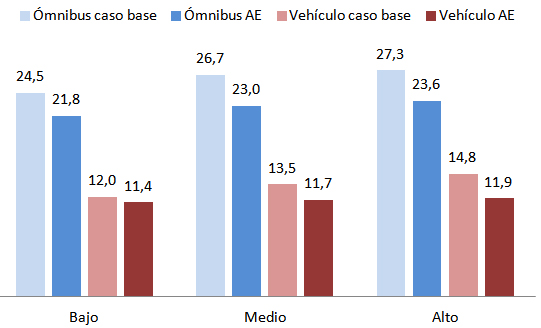
\includegraphics[width=0.7\linewidth]{Figures/duracion_viajes}
	\caption{Comparación de la duración en minutos de los viajes para ómnibus y otros vehículos en el recorrido completo del corredor Garzón para los diferentes tipos de tráfico.}
	\label{fig:duracion_viajes}
\end{figure}

Como se aprecia en el gráfico el algoritmo mejora la duración de los viajes tanto de ómnibus como de otros vehículos en los tres tipos de tráfico estudiados. Como cabía esperar aumenta la duración del viaje al aumentar el tráfico, aunque un resultado interesante es que la duración original de los viajes cuando el tráfico es bajo es casi igual a la duración de los viajes con tráfico alto luego de ejecutar el algoritmo.
Para ómnibus tenemos 24.5m y 23.6m y  para otros vehículos 12.0m y 11.9m. 



\subsection{Detalles del escenario alternativo}
Los cambios propuestos incluyen eliminación de paradas, semáforos, pasajes peatonales y alternar paradas. Se estudiaron otras propuestas pero fueron descartadas por la poca viabilidad real de las mismas. Como por ejemplo construir calles paralelas a Garzón o nuevas reglas en los cruces como existen en otros países.




\subsubsection{Eliminación de paradas}
Se consideraron dos paradas a eliminar que cumplieran con algunas características, no fueran cercana a una calle principal y que existiera otra parada cercana. Por lo que la eliminación de la parada no afecte en demasía a la gente en un traslado mayor.
En este caso se selecciono la parada en la calle Ariel y Casavalle.



\subsubsection{Eliminación de pasajes peatonales}
Hay tres pasajes peatonales en el corredor con semáforos que detienen el tráfico, dos de ellos solo manejan una esquina (sin pulsador en funcionamiento) donde en el escenario alternativo se implemento solamente mediante un "Pare" en la calle transversal al corredor y el otro es netamente peatonal frente a la Facultad de Agronomía que fue totalmente eliminado. Una opción que mantiene los pasajes peatonales así como también los resultados obtenidos en el escenario alternativo sería implementar el pasaje peatonal por encima del corredor. Al eliminar los pasajes peatonales se aumenta la velocidad media de todo el transporte.

\subsubsection{Alternar paradas}

Uno de los problemas del ómnibus es su baja aceleración por lo que cada vez que este frena en un semáforo o en una parada demora en retomar una velocidad aceptable. Por tanto al reducir la cantidad de paradas que un ómnibus tiene que hacer se mejora la velocidad promedio.
La linea G es la que recorre a Garzón de punta a punta, esta línea es cubierta por las empresas Coectc y Cutcsa. Una posibilidad de alternancia de paradas consiste en dividir las paradas por empresa y compartir las ganancias del corredor u otro método para equiparar el pasaje transportado. 

\begin{figure}[H]
	\centering
	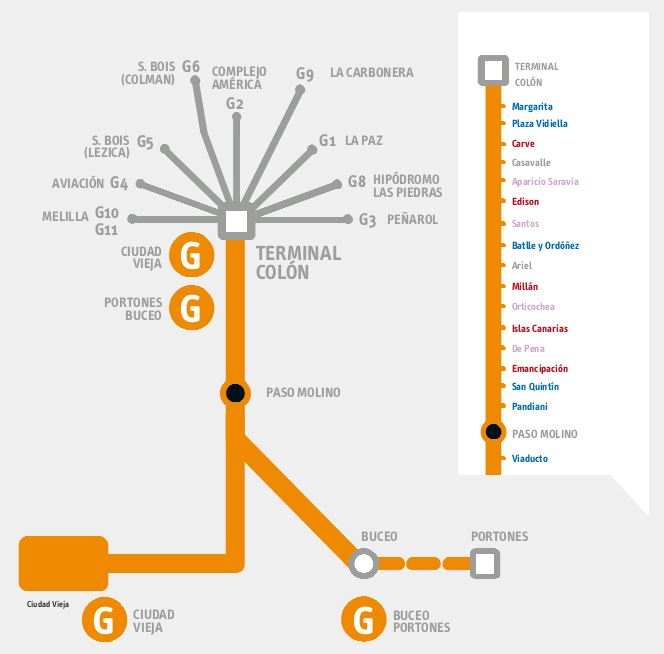
\includegraphics[width=0.7\linewidth]{Figures/paradas_alternativas}
	\caption{Gráfico de paradas alternativas. Gris: Parada Eliminada. Azul: linea G de Coectc y de Cutcsa. Rojo: linea G de Coectc. Violeta: G de Cutcsa. - Imagen original extraída de montevideo.gub.uy}
	\label{fig:paradas_alternadas}
\end{figure}

Una empresa se detendrá en las paradas pares y la otra en las impares y algunas de mayor aglomeración de pasaje/tiempo serán realizadas por las dos. Cada empresa viajará por el corredor a 4 minutos (como en la actualidad) Si se reduce el numero de paradas que hace un ómnibus, aumentará su velocidad promedio y al cubrir las paradas entre las dos empresas no se deberá resentir en demasía el servicio ya que la disminución de la frecuencia en una parada se contrarresta con el aumento promedio de velocidad.

Este cambio es el que mas aumenta la velocidad media y tal vez es uno de los mas sencillos de implementar en la realidad.



\subsubsection{Cambio básico de semáforos}
Al hacer el revelamiento de los datos se encontró que en todas las intersecciones en donde una línea de ómnibus que circula por el corredor tiene un viraje a la izquierda, se hace detener el tránsito de la derecha de la misma, cada vez que el corredor central tiene la luz verde. Esto no parece tener mucho sentido ya que podrían seguir circulando por el corredor sin ningún tipo de problema, el carril que hay que detener es el de la izquierda del ómnibus cuando una linea dobla a la izquierda pero no los dos carriles al mismo tiempo.

No se tiene conocimiento si esto corresponde a un error en la configuración, un tema de costos o facilidad para manejar los dos semáforos de los carriles paralelos juntos. Al suceder en varias intersecciones y para los dos lados se mejora la velocidad promedio de los autos que circulan por los dos carriles.

Este cambio se aplico en las siguientes intersecciones:
\begin{itemize}
	\item Islas Canarias: dobla línea 409 hacia la izquierda, orientado a Colon.
	\item Camino Ariel: doblan líneas como la  2 y la 148 hacia la izquierda, orientado a Paso Molino 
	\item Camino Casavalle: dobla línea 174 hacia la izquierda, orientado a Paso Molino 
\end{itemize}

\subsubsection{Resumen}
Lo interesante del resultado obtenido de esta modificación es que aumenta la velocidad promedio de los vehículos y disminuye la de los ómnibus. Aunque igualmente aumenta el fitness. 

En la siguiente tabla se detallan los cambios realizado con la mejora asociada, comparando los valores para el tráfico medio. Estos cambios son acumulativos, por lo que se hacen uno después del otro . Luego se detallan los resultados obtenidos para el tráfico bajo y alto.


\begin{table}[H]
	\renewcommand{\arraystretch}{1.2}
	\caption{Valores del escenario alternativo con su velocidad promedio ómnibus (vpb) y velocidad promedio vehículos(vpv) comparando el fitness para el tráfico medio }
	\label{table:resultado_alternativo}
	\centering
	\begin{tabular}{p{3.5cm}p{2.5cm}p{2.5cm}p{2cm}p{2cm} }
		\hline
		&
		$vbp(km/h)$& 
		$vvp(km/h)$ & 
		Fitness &
		Mejora(\%)
		\\ 
		\hline
		Base & 14.59  & 28.81& 12.05 & -\\
		Eliminar Paradas & 15.44  & 29.03& 12.35 & 2.4\\
		Eliminar Peatonales  & 16.02  & 29.32& 12.59 & 4.4\\
		Paradas alternadas  & 19.17  & 28.88& 13.34 & 10.7\\	
		Cambio reglas  & 18.50  & 29.70& 13.39 & 11.1\\				
		\hline
	\end{tabular}
\end{table}




\begin{table}[H]
	\renewcommand{\arraystretch}{1.2}
	\caption{Mejoras obtenidas para las velocidades promedio de los omnibus(vpb) y de otros vehiculos (vpv) en el escenario alternativo para distintos tipos de tráficos }
	\label{table:mejoras_trafico_alternativo}
	\centering
	\begin{tabular}{p{3.5cm}p{2.5cm}p{2.5cm}p{2cm}p{2cm} }
		\hline
		&
		$vbp(km/h)$& 
		$vvp(km/h)$ & 
		Fitness &
		Mejora fitness(\%)
		\\ 
		\hline

		Tráfico Bajo & 20.72  & 33.18 & 14.97 & 11.5\\
		Tráfico Medio & 18.50  & 29.70& 13.39 & 11.1 \\
		Tráfico Alto  & 18.60  & 27.17& 12.7 & 12.6\\		
		\hline
	\end{tabular}
\end{table}

\subsection{Resultados de la evaluación sobre el escenario alternativo}

Al comparar los resultados obtenidos se aprecia claramente que cuanto mas densidad de tráfico mayor es el porcentaje de mejora. Ademas un resultado interesante es que las diferencias entre los valores de los distintos tipos de tráfico se redujo.

Esto significa que el recorrido de un ómnibus por Garzón pasa de demorar 26,7 minutos a 17,8 minutos y un auto de demorar 14,5 minutos a 11.5 minutos con una densidad de tráfico media. 



\begin{table}[h]
	\renewcommand{\arraystretch}{1.2}
	\caption{Mejoras obtenidas al aplicar el algoritmo sobre el escenario alternativo. Comparando las velocidades de ómnibus(vpb), otros vehículos(vpv) y el fitness con cada tipo de tráfico contra el caso base o realidad actual.}
	\label{table:mejoras_trafico_alternativo_algoritmo}
	\centering
	\begin{tabular}{cccccccc}
		\hline 
		Tráfico& 
		$vbp(km/h)$& 
		$vpv(km/h)$&
		\multicolumn{2}{c}{Fitness}&  & 
		\multicolumn{2}{c}{Mejora fitness (\%)}\\  \cline{4-5} \cline{7-8}&     &     & \multicolumn{1}{c}{Promedio} & \multicolumn{1}{c}{Mejor} &  & \multicolumn{1}{c}{Promedio} & \multicolumn{1}{c}{Mejor} \\ \hline

		Bajo & 23.15$\pm$0.36 & 34.43$\pm$0.33 & 15.99$\pm$0.08 & 16.10 & & 19.1& 19.90 \\
		Medio & 21.83$\pm$0.50  & 33.89$\pm$0.22 & 15.47$\pm$0.09& 15.65 & & 28.3 & 29.87\\
		Alto & 21.46$\pm$0.54  & 33.41$\pm$0.38 & 15.24$\pm$0.19& 15.50 & & 34.8 & 37.10\\	
		\hline		    
	\end{tabular}
\end{table}


\subsection{Variación de la función de fitness}

La función fitness (\ref{eq:funcion_fitness}) utilizaba los pesos x = y = 1 lo que representa un balance equitativo  para ómnibus y vehículos.

%Por un cruce de Garzón pasan cada hora:
%70 ómnibus , si aproximamos con 23 personas= 1610 personas por hora
%800 autos, si aproximamos  2 personas por vehículo nos da 1600 personas por hora.
%Una cantidad similar  pasan por el cruce en ambos medios de transporte por lo que no existe una tendencia a favor de una sobre la otra, se podría aproximar que 50\% eligen el ómnibus y 50\% el auto.

Estos pesos pueden ser variados en función de lo que se necesite, por lo que se realizaran pruebas con dos tipos de pesos para comparar como varían las velocidades cuando se da mas peso a un tipo de vehículo sobre el otro.


\subsubsection{Prioridad ómnibus}
En este caso se le dará mas prioridad a los ómnibus, esto se sostiene en el hecho que uno de los objetivos buscados por la IMM  es que se utilice mas el transporte colectivo como parte de su plan de movilidad urbana \citep{PlanMovilidad}. Con la premisa que al mejorar la duración del viaje en ómnibus relativo al del auto por el corredor las personas que utilizan auto para sus viajes opten por el transporte colectivo.

Por tanto vamos a experimentar cambiando los pesos de la función fitness con un peso de 70\% para los ómnibus y 30\% al resto de los vehículos.


\subsubsection{Prioridad a otros vehículos}

En este caso, le damos 70\% del peso a los vehículos y 30\% a los ómnibus. Es el caso opuesto al anterior y servirá para poder comparar como varían los valores de las velocidades.

\subsubsection{Resultados}

La siguiente tabla compara las velocidades promedio de ómnibus y vehículos para los tres tipos de pesos que se probaron y por cada tipo de tráfico.  El caso 50-50 es el caso base donde los pesos son iguales, 70-30 es el caso con mas prioridad para los ómnibus y el 30-70 mas prioridad a los otros vehículos. Se analiza cuanto varían las velocidades de omnibues (var. vpb) y otros vehículos(var. vpv) comparando contra el caso 50-50 de cada tipo de tráfico.


\begin{table}[H]
	\renewcommand{\arraystretch}{1.2}
	\caption{Modificación de los pesos para ómnibus (pb) y para otros vehículos (pv) en la función fitness. Analizando las variaciones en la velocidad promedio de ómnibus (vpb),  otros vehículos (vpv) y fitness. }
	\label{table:analisis_fitness}
	\centering
	\begin{tabular}{p{1cm}p{1.2cm}p{1.8cm}p{1.8cm}p{1.8cm}p{1.2cm}p{1.2cm}p{1.2cm} }
		\hline
		Trafico &
		pb(\%) pv (\%)& 
		vpb & 
		vpv &
		fitness &
		var. \newline vpb(\%) &
		var. \newline vpv(\%) &
		var. \newline fitnesss(\%)
		\\ 
		\hline
		& 50-50  & 17.92$\pm$0.18 & 34.30$\pm$0.40 & 14.50$\pm$0.14  &- & - & -\\		
		Bajo & 70-30  & 17.93$\pm$0.23 & 34.06$\pm$0.17 & 12.65$\pm$0.11  & +0.07 & -0.70 & -12.79\\		
		& 30-70 & 17.55$\pm$0.23 & 34.71$\pm$0.21 & 16.42$\pm$0.10  & -2.06 & +1.18 & +13.21\\
		\hline
		
		& 50-50  & 16.95$\pm$0.32 & 33.29$\pm$0.29 & 13.95$\pm$0.15  &- & - & -\\		
		Medio & 70-30  & 17.29$\pm$0.27 & 33.08$\pm$0.14 & 12.24$\pm$0.12  & +2.0 & -0.62 & -12.30\\		
		& 30-70 & 16.71$\pm$0.42 & 33.79$\pm$0.31 & 15.92$\pm$0.11  & -1.41 & +1.49& +14.11\\
		
		\hline
		& 50-50  & 16.51$\pm$0.60 & 32.90$\pm$0.25 & 13.72$\pm$0.17  &- & - & -\\		
		Alto & 70-30  & 16.72$\pm$0.14 & 32.79$\pm$0.26 & 13.75$\pm$0.07  & +1.24 & -0.33 & +0.19\\	
		& 30-70 & 15.48$\pm$0.42 & 33.20$\pm$0.25 & 15.49$\pm$0.16  & -6.23 & +0.92 & +12.87\\
		\hline
			
				

		

	\end{tabular}
\end{table}


Los resultados indican que al variar los pesos de la función fitness las velocidades promedio de los vehículos se ve afectada. En el caso de dar mas prioridad a los ómnibus se produce como cabía esperar un aumento en su velocidad promedio y una leve baja en la velocidad promedio del resto de los vehículos. Cuando el tráfico es bajo este cambio casi no aumenta la velocidad de los ómnibus, una explicación posible de este comportamiento es que ya se llego a un limite máximo y no se puede mejorar mas.

Al dar mas prioridad a los otros vehículos se produce un aumento en su velocidad y una disminución en la velocidad de los ómnibus la cual es muy evidente en el caso de tráfico alto. Este resultado permite apreciar como estos valores son fuertemente afectados por la densidad de tráfico que se estudie.

En general las variaciones en las velocidades no son grandes pero suficientemente apreciable para tener cierta libertad al plantear distintos objetivos que tiendan a favorecer un tipo u otro de vehículos.


\subsection{Eficiencia computacional}

Se realiza un estudio de la eficiencia computacional del algoritmo para analizar los tiempos de ejecución cuando se usan varios procesadores y como se comporta su capacidad de paralelismo.

Se evalúan nueves ejecuciones del algoritmo; tres con con cada tipo de tráfico: alto, medio y bajo. Para estudiarlo en diferentes contextos. El algoritmo utiliza 32 hilos de ejecución por lo que utilizamos esa cantidad de procesadores.

Las pruebas fueron realizadas sobre el node40 del Cluster Fing que tiene las siguientes características:

\begin{itemize}
	\item Modelo: HP Proliant DL585
	\item Procesador: AMD Opteron 6272 2.09GHz
	\item Memoria: 48GB
	\item Cores utilizados: 32
\end{itemize}





El speedup(S) mide la mejora de rendimiento de una aplicación al aumentar la cantidad de procesadores comparando con el rendimiento al usar un solo procesador.
\begin{equation}
\label{eq:funcion_speedup}
S = \frac{T_1}{T_N}
\end{equation}
Donde ${T_1}$ es el tiempo de ejecución del algoritmo serial o secuencial, y ${T_N}$ el tiempo del algoritmo ejecutado sobre N procesadores.
\newline

La eficiencia computacional (E) corresponde al valor normalizado del speedup (entre 0 y 1) respecto a la cantidad de procesadores. Los valores cercanos a uno indican una alta eficiencia computacional.
\begin{equation}
\label{eq:funcion_eficiencia}
E = \frac{T_1}{N*T_N} = \frac{S}{N}
\end{equation}



\begin{table}[H]
	\renewcommand{\arraystretch}{1.2}
	\caption{Análisis de eficiencia computacional comparando los tiempos de ejecución en serial y paralelo en minutos. }
	\label{table:analisis_speedup}
	\centering
	\begin{tabular}{p{2.5cm}p{2.5cm}p{2.5cm}p{2.5cm}p{2.5cm} }
		\hline
		
		Instancia& 
		Serial(m) & 
		Paralelo(m) &
		Speedup &
		Eficiencia
		\\ 
		\hline
		bajo1  & 1572 & 59 & 26.64 & 0.83\\
		bajo2  & 1571 & 59 & 26.62 & 0.83\\
		bajo3  & 1183 & 44 & 26.88 & 0.84\\
		
		medio1  & 3002 & 119 & 25.22 & 0.78\\
		medio2  & 2195 & 82 & 26.76 & 0.83\\
		medio3  & 3007 & 120 & 25.05 & 0.78\\
		
		alto1  & 2920 & 110 & 26.5 & 0.82\\
		alto2  & 4365 & 183 & 23.85 & 0.74\\
		alto3  & 4276 & 177 & 24.15 & 0.75\\
		\hline
		  &  & Promedio & 25.7$\pm$1.1 & 0.80$\pm$0.03\\
		
		\hline
	\end{tabular}
\end{table}


El algoritmo paralelo logra una mejora sustancial en los tiempos de ejecución con un valor promedio del speedup de 25.7  y  eficiencia promedio de 0.8, lo que podemos considerar como buenas métricas.

\begin{figure}[h]
	\centering
	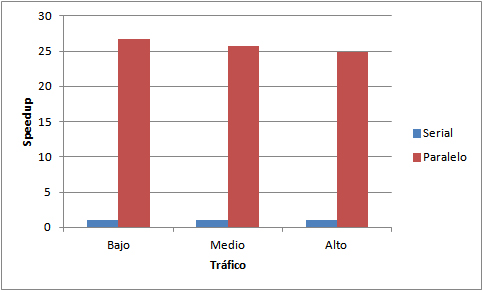
\includegraphics[width=0.7\linewidth]{Figures/speedup1}
	\caption{Comparación de los speedup promedios para cada tipo de tráfico.}
	\label{fig:speedup1}
\end{figure}

En la gráfica se observa como a medida que aumenta el tráfico disminuye el speedup esto sucede por que esta influenciado por los accesos al disco duro, al tener mas autos circulando en la simulación se tiene que leer y escribir mas información en los archivos lo que aumenta el tiempo de ejecución del algoritmo, aunque como se ve esto no tiene un gran impacto.